\documentclass[12pt, oneside]{extbook} % the document type needs to be change
\usepackage{geometry}
\usepackage{listings}
\usepackage{graphicx}
\usepackage[utf8]{inputenc}
\usepackage[T1]{fontenc}
\usepackage[italian]{babel}

\geometry{
    top = 1.5cm,
    bottom = 1.5cm,
    left = 2cm,
    right=2cm,
}

\begin{document}

\chapter*{Secure protocols and overlay VPNs}

\section{Recap: protocolli di sicurezza di rete}
Abbiamo visto che i meccanismi base di IP sono insicuri, non c'è nulla.
\\Abbiamo discusso alcuni possibili meccanismi di difesa
\begin{itemize}
    \item 802.1X auth
    \item firewalls
    \item ACL
\end{itemize}
abbiamo anche visto come la crittografia può permetterci di rendere sicuri i protocolli, vediamo ancora come usare i tool crittografici: tramite questi, tutto quello che non viene offerto dal protocollo di base può essere fatto con la crittografia simmetria / asimmetrica.
\\Definiamo gli standard che usano le funzionalità crittografiche, applicate a diversi livello dell'ISO/OSI

\section{Livello applicativo: SSH}
SSH serve per avere un accesso remoto sicuro ad un server, dobbiamo accedervi perché non vi abbiamo accesso fisico.
\\Ci sono gli stessi problemi di prima:
\begin{itemize}
    \item il server a cui ci loggiamo è quello giusto?
    \item username e password mandate sul canale vengono captate?
    \item data integrity?
\end{itemize}
\texttt{telnet} era un protocollo usato per la comunicazione fra due host, ma fu progettato senza minimamente pensare alla sicurezza, infatti ci sono diversi problemi.
\\Si è cercato di fare delle patch di sicurezza a \texttt{telnet}, ma era meglio ripartire da 0 ed è quello che è accaduto con telnet.
\\SSH è un protocollo di sicurezza per il login remoto, è formato da una serie di protocolli tra cui i 3 principali sono:
\begin{itemize}
    \item Il protocollo di transport layer
    \item User auth protocol
    \item Connection protocol
\end{itemize}
ci sono svariate implementazioni OS di ssh, una delle più famose in Linux è \texttt{openssh} che offre diversi servizi:
\begin{itemize}
    \item Cifratura, autenticazione e data integrity
    \item trasferimento di file sicuro (\texttt{scp})
    \item forwarding X session
    \item forwarding porta
    \item ...
\end{itemize}
\subsection{SSH transport layer}
Gira tipicamente su tcp/ip, la secure shell ha bisogno di una consegna sicura del messaggio quindi si usa tcp piuttosto che udp.
\\Il layer di trasporto gestisce la parte iniziale dell'handshake, alla fine si ottiene una shell sicura per poter creare altri canali
\subsection{User Authentication}
Ci sono diversi modi per autenticarsi con ssh
\begin{itemize}
    \item password based
    \item public key
    \item keyboard interacting
    \item GSSAPI authentication
\end{itemize}

\subsection{SSH conenction layer}
Dopo l'handshake, si possono usare diversi servizi come ad esempio \texttt{sftp}, \texttt{scp} etc... che si possono negoziare e far partire dopo l'handshake iniziale.
\\SSH usa diversi algoritmi di cifratura, molti dei quali simili a quelli usati da TLS: all'atto dell'handshake, si negoziano gli algoritmi da usare etc..\\
\begin{figure}[h!]
    \centering
    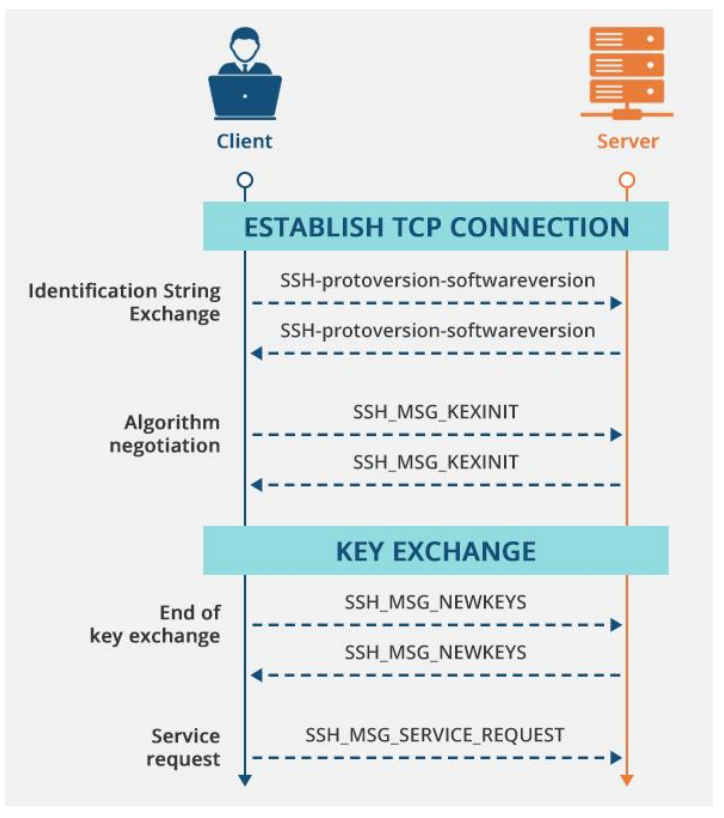
\includegraphics[scale=0.5]{../../immagini/ssh_hs}
\end{figure}\\\\
La prima volta che ci si connette via ssh, viene ricevuta dal client lo SHA256 della chiave pubblica del server di ECDSA: ssh non usa certificati x509 e quindi siccome non c'è una CA di terza parte non possiamo certificare l'autenticità del server.
\\Dobbiamo certificare manualmente l'autenticità del server: la connessione è critica, è la prima volta che il server manda la sua chiave pubblica ed è fondamentale.
\\Se qualcuno è nel mezzo della connessione, è non protetta e quindi può fare eavsedropping etc...
\\Come possiamo essere sicuri che la chiave è corretta?\\Verificando se il fingerprint corrisponde con quella del server e c'è un comando apposito: le chiavi del server sono tutte in \texttt{/etc/ssh/...}.
\\Possiamo quindi loggarci con la password, fatto una volta non verrà più richiesto di assicurarsi se ci si fida dell'identità associata alla chiave pubblica.
\\Lo scenario è ragionevole per non avere un certificato X509 per ogni server a cui connettersi, il che rende il tutto più scalabile ma non è applicabile a server web, cosa accade se nei prossimo login non si verifica questa associazione?
\\C'è un grande warning dal client: ricevo una chiave pubblica diversa, spesso però non è un qualcosa di malevolo perché magari semplicemente sono state rigenerate le chiavi, quindi per sbloccarsi occorre cambiare l'associazione fra identità e chiave.

\subsubsection{Mutual public key auth}
Il client si autentica per default usando username e password.
\\Per default, utenti di root non si possono loggare, sappiamo che nella catena di sicurezza gli utenti sono quelli più deboli perché scelgono password deboli, quindi il server si autentica con chiave pubblica sempre, ma il client no.
\\Dobbiamo abilitare lo scenario di autenticazione con chiave pubblica del client: si può fare durante l'handshake oppure cambiando il file di configurazione di ssh.
\\Serve una coppia di chiavi per il client, che vanno generate esplicitamente, tramite \texttt{ssh-keygen} e viene sempre creato un file nella home directory.
\\Il problema è lo stesso del server, la chiave non è certificata e quindi va resa sicura per il server o meglio va installata nel server
\begin{itemize}
    \item si può fare manualmente
    \item si concatenano tutte le chiavi a cui è permesso fare PKA nel file \texttt{authorized\_keys} per l'utente sul server.
    \\Si può fare copiando il file sul server oppure col comando \texttt{ssh-copy-id}
\end{itemize}

\section{Transport layer: TLS}
Anche se è possibile incapsulare dati IP raw in SSH, sipuò pensare di usarlo per proteggere il traffico IP, manon è l'approccio migliore.
\\Se dobbiamo rendere sicuri tutti i protocolli applicativi come HTTP, dobbiamo rifare lo stesso approccio per tutti i protocolli.
\\Possiamo quindi far si che meccanismi di sicurezza siano in layer sotto quelli applicativi ed esposti come servizi.
\\TLS è un protocollo fra il livello 5 e 4, è una protezione per applicazione perché è per singola porta.
\\Quindi, gli obiettivi di TLS sono:
\begin{itemize}
    \item stabilire una sessione, mediante la fase di handshake dove si concordano algoritmi, si condividono segreti e si fa autenticazione
    \item trasferire dati applicativi, fornendo confidenzialità (cifratura simmetrica) ed integrità (HMAC) 
\end{itemize}
TLS gestisce i record protocol, generati a partire dai dati applicativi, usando diverse operazioni:
\begin{itemize}
    \item frammentazione: a livello applicativo di TLS, un frammento può essere massimo di 16384 byte
    \item compressione: veniva fatta una compressione lossless, ma dal 2012 in seguito all'attacco CRIME è stata tolta.
    \item MAC: calcolo del MAC, usando la chiave detivata dai parametri di sicurezza condivisi e la funzione di hash negoziata
    \item encryption: da fare dopo il MAC (altrimenti è letale per la sicurezza), quindi si applica sia al frammento compresso che al MAC.
    \\È fatta usando algoritmi di crittografia simmetrica, usando una chiave diversa da quella del MAC
\end{itemize}
Non si usa un numero di sequenza in TLS in quanto è implicito quello di TCP (per l'anti replay), nel caso di UDP è stato standardizzato apposta (8 byte DTLS).
\\Prima di far partire lo scambio dati si fa un handshake, fornisce gli stessi servizi di ssh:\\
\begin{figure}[h!]
    \centering
    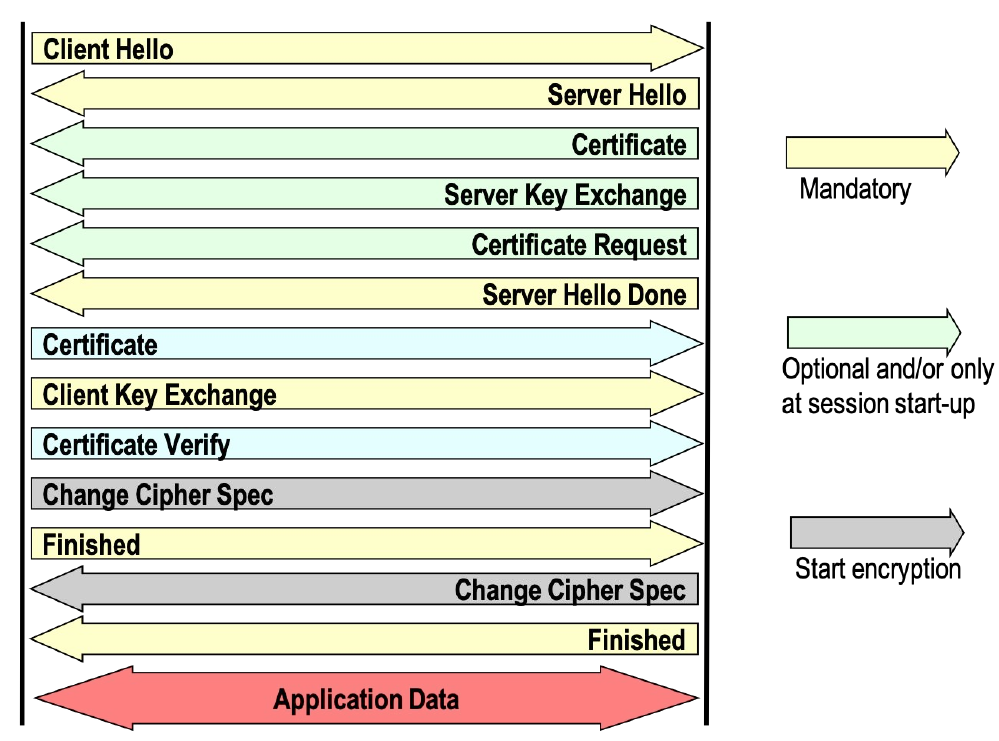
\includegraphics[scale=0.5]{../../immagini/tls_hs}
\end{figure}
\\\\L'handshake si fa quando si crea una sessione di TLS ma anche quando si vogliono rinegoziare le chiavi, da una chiave master si generano tutte le sotto-chiavi.
\\Gli obiettivi dell'handshake sono vari:
\begin{itemize}
    \item negoziazione sicura dei segreti condivisi
    \item autenticazione opzionale
    \item negoziazione affidabile
\end{itemize}

\section{Livello rete: IPSec}
IPsec usato per rendere sicura la comunicazione su IP. Gli obiettivi sono gli stessi di TLS, ma ci sono delle differenze
\begin{itemize}
    \item IPsec è una suite di protocolli, combinazione di diversi standard (ESP, AH etc...)
    \item operano su due livelli diversi, IPsec è a layer 3 quindi con IPsec si protegge l'host, mentre TLS protegge l'applicazione
    \item in IPsec ci sono le security associations
    \item IPsec ha delle policy di sicurezza esplicite
    \item IPsec ha diverse modalità di operatività che vanno definite
    \item mentre TLS spesso è implementato user space, IPsec è kernel space
\end{itemize}

\section*{LAB 007}
IL motivo per cui l'HTTPs downagrade è ancora possibile è dovuta alla possibilità di fare ridirezione su https quando si ci collega ad un sito che supporta ssl ma per default il brownser prepende all'URL http.

\section{Attacchi a TLS}
\subsection{HTTPs downgrade}
L'attaccante riesce a mettersi nel mezzo di una comunicazione HTTPs e rimuove la "s" fra se stesso e la vittima e forwarda i pacchetti con una sessione HTTPs reale col server.
\\Possiamo anche metterci nel mezzo ma anche fare reply come il target server ma senza forzare l'uso di TLS nella comunicazione.
\\Funziona davvero? Come fa il browser della vittima a non rendersi conto che viene rimosso TLS?
\\Il problema è storico, in quanto nel passato i siti web erano ibridi, quindi permettevano http per il sito, si è poi deciso di usare ancora http magari per la home page ed oggi è ancora così.
\\Ad esempio per configurare un server https serve la ridirezione esplicita, ma se il browser può mandare una http get in chiaro l'attacco funziona.
\\L'attacco può essere fatto così
\begin{itemize}
    \item ci mettiamo nel mezzo fra la vittima ed il router
    \item redirigiamo il traffico da un certo sito web ad un proxy interno
    \item non redirigiamo il traffico https
    \item ...
\end{itemize}
Si può mitigare l'attacco tramite HSTS, meccanismo per il cui il server informa il browser che la connessione al sito dovrebbe sempre usare ssl/tls.
\\Quindi l'header HSTS è dentro la richiesta http dentro cui il server specifica che supporta solo https.
\\Ci sono delle limitazioni
\begin{itemize}
    \item la prima richiesta rimane non protetta
    \item c'è un timeout, alla fine del quale viene ricevuto un altro HTST header
    \item non tutti i client usano HSTS
\end{itemize}
alcuni siti più noti usano una lista pre-caricata di nomi, ma non copre tutti i siti.

\subsection{Renegotiation attack}
TLS permette al client o al server di iniziare la renegoziazione in un nuovo handshake, che stabilise nuovi parametri crittografici.
\\Sfortunatamente, siccome il nuovo handshake avviene nel canale protetto stabilito precedentemente, non c'è una connessione crittografica fra i due.
\\Questo fa si che un ataccante, se in grado di intercettare la connessione del client, possa iniettare il suo traffico come prefisso dell'interazione fra client e server.

\subsection{CRIME, POODLE, BEAST ad Hearthbleed}
CRIME è un attacco che sfrutta la compressione: un testo come AAAABC, viene compresso in 4ABC (a seconda dell'algoritmo usato), quindi una volta cifrato risulta in un ciphertext di 4 byte sempre.
\\Questo può portare un attaccante a scoprire il valore del plaintext, è un attacco del 2012 ma in realtà era già stato detto nel 2002 ed affligge in generale tutti gli algoritmi di compressione.
\\\\
Il Padding Oracle si applica al modo di operare del CBC, dove "l'oracolo" (che spesso è il server) fornisce informazioni sul fatto che il padding per un messaggio cifrato sia corretto o no.
\\Permette all'attaccante di decifrare i messaggi senza conoscere la chiave segreta.
\\Infatti, quando viene fatta la decifratura, viene validato il padding e se c'è un errore il server restituisce il messaggio di "invalid padding", quindi un attaccante che riesce ad osservare i due blocchi di ciphertext consecutivi C$_0$ e C$_1$ può testare se il plaintext P$_1$ è uguale ad x scegliendo il prossimo plaintext P$_2$ tale che
\begin{equation}
    P_2 = x + C_0 + C_1
\end{equation}
Siccome C$_2$ = E(C$_1$ + P$_2$) = E(C$_1$ + x + C$_0$ + C$_1$) = E(C$_0$ + x) che sarà uguale a C$_1$ se x = P$_1$.
\\\\
L'hearthbleed è un bug alla libreria crittografica \texttt{openssl} che è dovuta ad un buffer overflow, che faceva si che il TLS hello fosse simile ad un ICMP echo e quindi permetteva leak di username e password.

\section{Overlay VPN}
Una VPN estende una rete privata, permettendo agli utenti di mandare traffico fra reti pubbliche come se fossero connessi nello stesso segmento di rete.
\\È una rete privata, quindi nessuno dall'"esterno" può accedere al traffico di rete.
\\Cifratura ed integrità sono comuni, nella overlay VPN sono obbligatorie ma in altri tipi di VPN non lo sono, ad esempio le intra-AS VPN non forzano la cifratura.
\\L'overlay VPN ha una topologia costruita su una topologia esistente non sicura, come ad esempio Internet.
\\La rappresentazione grafica è la seguente:\\
\begin{figure}[h!]
    \centering
    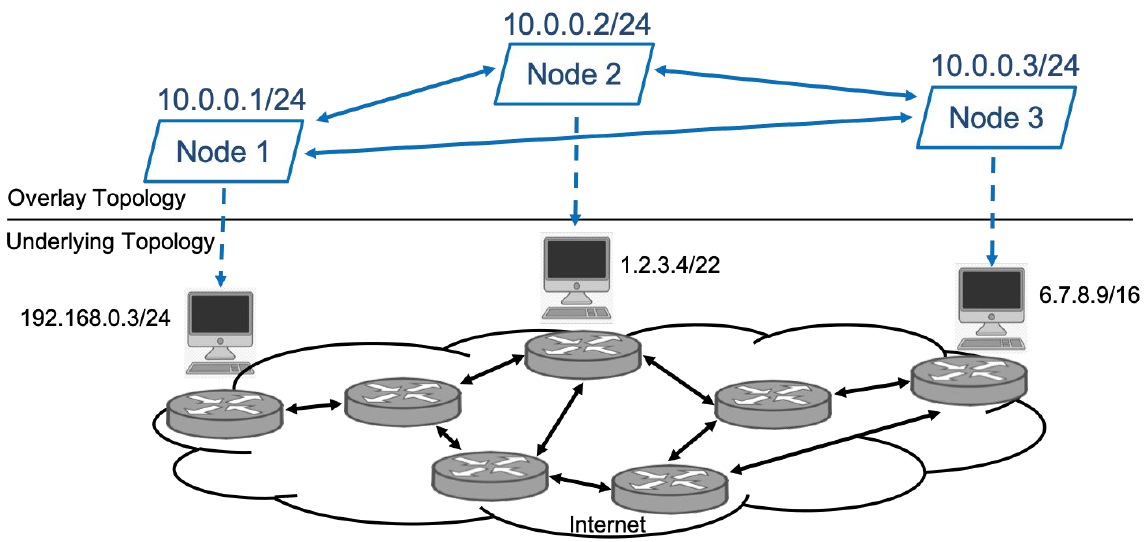
\includegraphics[scale=0.5]{../../immagini/vpn_overview}
\end{figure}\\\\
costruiamo quindi la nostra topologia virtuale sulla cima di un'altra rete.
\\Ci sono 2 problemi da risolvere
\paragraph{Creare una rete privata} Come realizzare una rete privata che consiste in nodi deployati su reti diverse, è un problema di addressing e routing.
\\L'addressing si risolve, il problema è il routing: serve poter raggiungere un nodo centrale che abbia un IP pubblico, che poi deve saper raggiungere i nodi privati, la soluzione di come parlare con i nodi è il \textbf{tunneling}.
\\Il tunneling è un concetto generico, in quanto si fa tunneling quando si incapsula un protocollo come payload di un altro\\ 
\begin{figure}[h!]
    \centering
    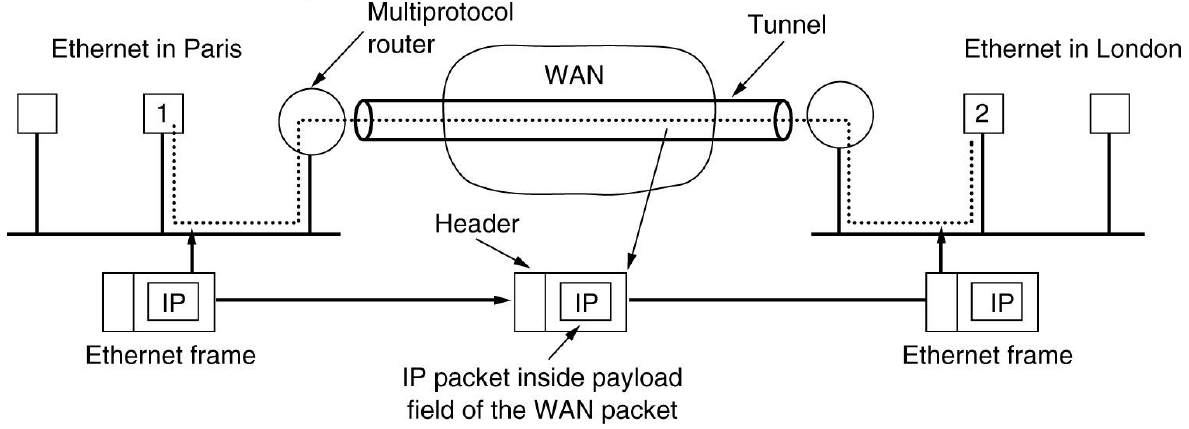
\includegraphics[scale=0.5]{../../immagini/vpn_tunnel}
\end{figure}\\\\
Per risolvere il problema, serve comunque avere un server con IP pubblico, il pacchetto esterno può raggiungere il secondo router, il pacchetto interno è in qualche modo nascosto e non viene visto dal router, i router fanno forwarding solo guardando l'header esterno.
\\Abbiamo quindi una rete virtuale, ma non è privata perché tutti i router nel percorso sono in grado di capire chi è il destinatario.\\

\paragraph{Problema 2: usare protocolli di sicurezza} Occorrono protocolli di sicurezza per incapsulare il traffico interno, non è solo un problema di integrità, encryption etc... ma anche di verifica di identità.
\\Possiamo avere diversi tipi di encryption + authentication, sia gateway to gateway ma anche host to host\\
\begin{figure}[h!]
    \centering
    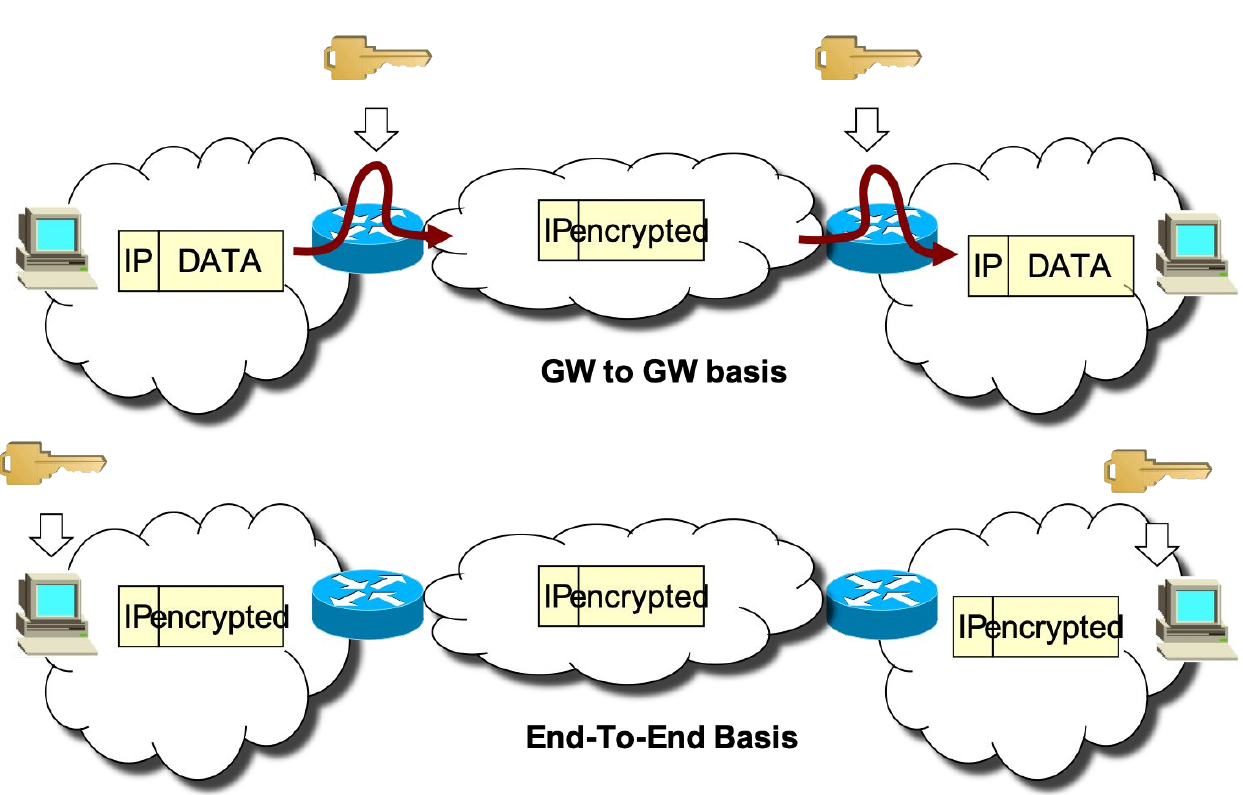
\includegraphics[scale=0.5]{../../immagini/vpn_types}
\end{figure}

\subsection{OpenVPN}
VPN lato user space con \texttt{openvpn}: tool open source per creare delle VPN.
\\Ha un protocollo costum, usa due canali uno per controllo ed uno per i dati, supporta sia tunneling UDP che TCP, lo scenario più comune è UDP tunneling.
\\Il canale di controllo usa TLS per negoziazione delle chiavi e autenticazione etc... e poi c'è lo scambio dati sull'altro canale, \texttt{openvpn} usa \texttt{openssl} ed offre un sacco di feature.
\\Un building block fondamentale di \texttt{openvpn} è il tun/tap driver:

\begin{itemize}
    \item un TUN driver è un device di rete point-to-point per tunneling IP.
    \\Quindi, le applicazioni possono usare questa interfaccia virtuale configurando le tabelle IP, il TUN manda i pacchetti IP allo user space dove un'altra applicazione è in ascolto ed è un modo per integrare in maniera trasparente \texttt{openvpn} con i programmi in esecuzione, non è \texttt{openvpn} l'applicazione che manda il traffico e quindi si aggiungono delle rotte che mandano il pacchetto per il TUN device in modo che sia \texttt{openvpn} che riceve il traffico.
    \\È un modo per "fregare" l'applicazione quando manda il traffico, quando \texttt{opevpn} riceve il pacchetto lo manda attraverso la vera NIC.
    \\Le applicazioni non se rendono conto, il sysadmin lo sa e configura le tabelle di routing
    \item un TAP: device di livello 2, mentre il TUN è di livello 3.
    \\Quindi, ad esempio possiamo fare tunneling di richieste broadcast etc...
\end{itemize}
Il funzionamento è il seguente:
\begin{figure}[h!]
    \centering
    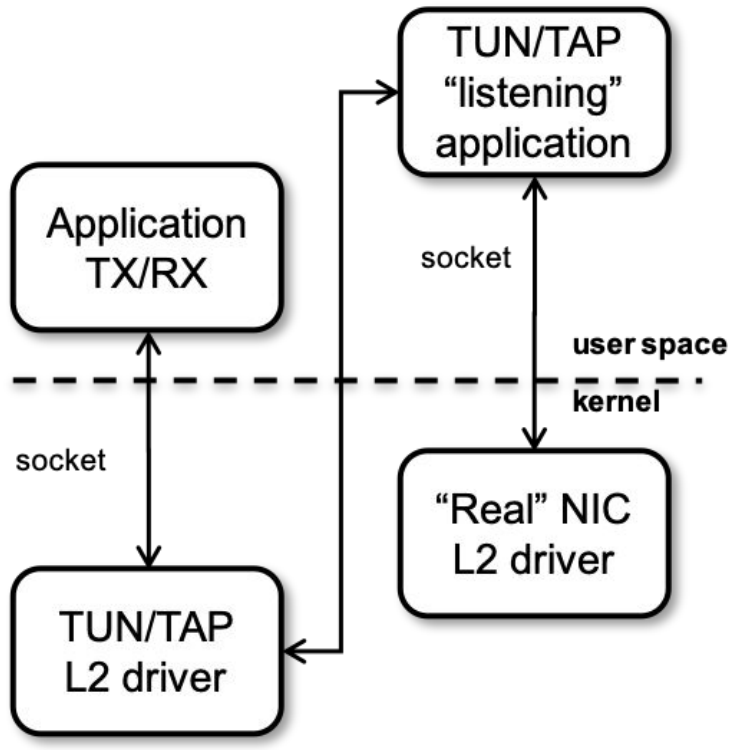
\includegraphics[scale=0.5]{../../immagini/tun_tap}
\end{figure}\\\\

È importante ricordare che \texttt{openvpn} è NAT friendly perché è un protocollo di tipo client/server, quindi il client parla per primo e se c'è una NAT è come un qualunque scambio client/server.

\subsubsection{OpenVPN PKI}
Abbiamo quindi l'openvpn server, che riceve il pacchetto con l'IP virtuale configurato dalla VPN, incapsulato in un TCP/UDP header oppure IP header, dove l'IP è quello reale della rete.
\\C'è un collegamento point-to-point, quindi serve solo conoscere l'IP dell'altro end.
\\Il PKI di \texttt{opevpn} usa TLS, da un punto di vista alto basta sapere questo, viene usato nell'handshake: il server usa una chiave pubblica per autenticarsi, il client può usare username e password ma anche certificati x509.
\\Se vogliamo fare nel modo migliore, dobbiamo mettere su il PKI con la CA etc..., che è un normale PKI x509 e possiamo usare un tool completamente compatibile con \texttt{openvpn} che è \texttt{easyRSA}, serve un certificato separato per client e server ed anche una CA master per certificare i coefficienti di DH.
\\Al server basta avere chiavi pubbliche e private ed il certificato che ha la chiave pubblica associata alla chiave privata usata per firmare gli altri certificati (quella quindi di root o della CA intermedia).
\\Se viene compromessa una chiave privata, c'è la revoca dei certificati classica di x509.
\\Possiamo creare quindi ACL basate sui client facilmente identificandoli con i common name all'interno dei certificati.

\subsubsection{OpenVPN protocol}
C'è una regola generale che dice che se UDP funziona va usato, altrimenti si usa TCP, ma in generale UDP è la scelta migliore quindi assumiamo che il layer 4 usato sia UDP da adesso in poi.
\\OpenVPN usa TLS, usato solo per autenticazione e per scambiare materiale per le chiavi, usiamo però UDP come layer 4 e TLS si aspetta di lavorare sotto TCP e c'è la versione apposita di TLS che è DTLS che non supporta diverse cose invece supportate da TLS.
\\OpenVPN usa TLS sul top di TCP ed implementano un meccanismo di ACK semplice per garantire la consegna.
\\Vengono usati due canali
\begin{itemize}
    \item un canale di controllo con TLS, usato allo start della connessione fra client e server
    \item un canale dati, incapsulato nello stesso tunnel udp, riconosciuto tramite l'header openvpn dove viene scambiato traffico enrcypted.
\end{itemize}
C'è una versione meno sicura di openvpn in cui le chiavi sono configurate staticamente (pre-shared).
\\Durante l'inizializzazione del canale, c'è il classico tls handshake, dove quindi si possono scegliere i chipersuite voluti, gli algoritmi di cifratura e autenticazione sono staticamente messi nel file di configurazione.

\section*{LAB 008}
La prima cosa da fare è crearsi la propria PKI, usiamo \texttt{easy-rsa}.
\\La prima cosa da fare è . ./vars per importare l'ambiente virtuale.
\\Buildiamo i certificati della ca con \texttt{./build-ca}, ogni cosa creata viene salvata nella directory keys.
\\In seguito, con \texttt{./build-key-server} col nome del server, siccome va trustata solo localmente va bene avere una CA "non trusted", si fa tutto automaticamente; lo stesso per i clients.
\\Serve poi creare i certificati per i coefficienti DH.
\\Ogni nodo ha una coppia di chiavi ed un certificato, il certificato del client sta solo sul client perché lo manda lui durante l'handshake.
\\Il certificato della CA sia sul server che sul client perché serve avere la chiave pubblica della CA e siccome è self signed serve installare la root CA in tutte le macchine che devono verificare le chiavi.
\\Nella topologia c'è un access gateway che è un client in \texttt{openvpn}, quindi può essere sfruttato dall'host connesso per entrare nella vpn.
\\I due nodi all'interno delle sotto-reti sono completamente ignari dell'esistenza della vpn.
\\Nel router CISCO abbiamo un'access list per matchare i pacchetti che passano.
\\Il modo migliore per poter scrivere i file di configurazione di \texttt{openvpn} è partire da quelli già presenti nell'applicazione, le opzioni più importanti sono
\begin{itemize}
    \item port: porta di ascolto del server, è la porta di destinazione del pacchetto tunneled verso il server;
    \item proto: tpc o udp
    \item dev
    \item ca: il path ai certificati
    \item cert
    \item key
    \item dh
    \item client: dice ad openvpn che siamo dei client 
    \item remote: da specificare in caso di nodo client
    \item server, il duale di client
    \item client\_to\_client
    \item push route
    \item route
    \item client\_config\_dir
\end{itemize}
Ci sono 3 diverse direttive di route
\begin{itemize}
    \item route è per la macchina locale
    \item push route è lo stesso, ma facciamo il push
    \item iroute influenza il routing della overlay: se dobbiamo mandare un pacchetto nella rete di overlay abbiamo bisogno delle informazioni relative.
    \\Il server è il forwarder della overlay network, è lui che manda i pacchetti nel tunnel e deve conoscere quale rete si trova dietro quale tunnel.
    \\Quindi, i client vengono confiugrati in modo che i pacchetti verso la vpn abbiamo come next hop l'indirizzo di un link point-2-point, quindi non ci saranno arp request.
    \\L'unico che deve conoscere informazioni sulla rete di overlay è il server perché la topologia è di tipo "hub and spoke"(??)
\end{itemize}
Per far partire \texttt{opevpn}, è possibile configurarlo anche per girare con \texttt{systemctl} oppure da shell
Test cases per verificare la configurazione:

\begin{itemize}
    \item (slides per il primo test case)
    \item secondo test case: client1 pinga tiny1 (rispetto alle slides).
    \\Tiny1 può essere raggiunto solo dal server in quanto è connesso via il router, servirebbe una destination NAT ma non è quello che vogliamo: la vpn non è solo raggiungere qualcuno in una rete privata, ma anche rendere sicura la comunicazione.
    \\Abbiamo aggiunto una regola di MASQUERADE sul server, quindi tiny1 vede un ping dall'IP pubblico 2.0.0.2, che è quello del server.
    \\La reply torna al server, viene de-nattato e inviato al client.
    \\Se non ci fosse stato il masquerade, ci sarebbe stato come indirizzo IP destinazione del echo reply 192.168.100.x, che era l'IP virtuale del server ed il router 2 non saprebbe come raggiungerlo (non ha la route) e quindi il pacchetto sarebbe discardato;
    \item test case 3: client1 pinga tiny2: il pacchetto interno ha dest address 10.0.0.100, la route sul server vpn per questo indirizzo è su tun0, ma ora il server ha due possibilità: ha un tunnel verso client 1 ed uno verso client2 ed è un problema di routing di overlay.
    \\Abbiamo scritto nel file di configurazione del client2 l'iroute, quindi il server sa che il pacchetto deve essere forwardato a client2 perché viene matchata la regola.
    \end{itemize}

\subsection{Interazione con NETFLITER}
Supponiamo di voler configurare un firewall sul server, abbiamo tutte le regole in drop e dobbiamo permettere alcune regole per far si che tutto funzioni:
\begin{itemize}
    \item partiamo con tutto in drop tramite iptables
    \item ora, tutti i collegamenti nella vpn non funzionano
    \item il primo layer è il tunnerl esterno, quindi vogliamo sbloccare la comunicazione per il control channel, ma facendo così sblocchiamo anche il data channel che è sullo stesso canale udp
    \item come prima cosa quindi, sblocchiamo con \texttt{iptables} udp sulla porta 1194 in input.
    \\Ora o usiamo lo state match con cui permettiamo solo le connessioni established oppure lo facciamo permettendo i pacchetti di risposta
    \item ora l'handshake iniziale parte, ma non basta.
    \\Quando viene decapsulato il pacchetto, vogliamo permettere che il pacchetto si accettato quando l'interfaccia di input sia tun0, in modo da riconoscere che il pacchetto appartiene alla vpn;
    \item occorre anche sbloccare i pacchetti da e verso tun0 ma in FORWARD, ovvero quelli che vanno verso i due tiny nelle sotto-reti private.
\end{itemize}

\section*{Lab09}
IP over GRE over IPses.
\\In questo esempio configuriamo una vpn staticamente, usiamo una gw2gw vpn: la modalità che usiamo è la tunnel mode, ovvero vogliamo incapsulare i pacchetti dentro altri pacchetti IP.
\\Un problema di IPsec è che non si possono usare indirizzi multicast, una soluzione è usare GRE quindi
\begin{itemize}
    \item creiamo un tunnel GRE fra i due gatweay
    \item usiamo IPsec in transport mode per protegge i pacchetti nel tunnel GRE
    \item le SA (Security Association) quindi si applicano ai pacchetti GRE
\end{itemize}
così possiamo incapsulare anche pacchetti multicast.
(slides per vedere come finisce il laboratorio)
Dobbiamo creare le due SAs per entrambe le direzioni, la cryptomap mescola la policy alla SA.

\end{document}
